
\begin{center}
%TODO: adequate caption
{\bf НЕЛОКАЛЬНАЯ КОНЕЧНОМЕРНАЯ РЕДУКЦИЯ УРАВНЕНИЯ КОЛЕБАНИЙ
МАЯТНИКА}


Т.И. Костина, Ю.И. Сапронов (Воронеж, ВГТУ, ВГУ)

\end{center}
\addcontentsline{toc}{section}{Костина Т.И., Сапронов Ю.И.\dotfill}

\vspace{3mm}

Колебания <<загруженного математического маятника>> (далее
<<маятника>>) описываются (см. [1]) уравнением
 $$
f(\varphi):=\frac{d^2 \varphi}{ds^2} + \lambda\,\sin(\varphi) = q\,,
\eqno{(1)}
 $$
где $t$ --- {\em время},  $\varphi = \varphi(t)$
--- {\em угол отклонения} маятника от положения равновесия, $\lambda$
--- параметр нагрузки, $q =q(s)$ --- {\em функция внешнего колебательного
воздействия}. Будем рассматривать это уравнение при периодических
краевых условиях с фиксированным периодом $2\,\pi$:
 $$
\varphi(t+2\,\pi)=\varphi(t)\,. \eqno{(2)}
 $$
Заметим, что колебания с периодом, отличным от $2\,\pi$, также
<<охватываются>> задачей (1)-(2) посредством масштабирующих
преобразований вида $\varphi\longmapsto \alpha\,\varphi$,
$t\longmapsto \beta\,t$, \ $\lambda\,\longmapsto \gamma\,\lambda\,$.

Задача  (1)-(2) определяет  экстремали {\em функционала
энергии}
 $$
V (\varphi, \lambda, q):= \frac
1{2\pi}\int\limits_0^{2\,\pi}\left(\frac{{\dot\varphi}^2}2+\lambda
(\cos\varphi - 1 ) + q\varphi\right)\,ds\,. \eqno{(3)}
 $$

С целью упрощения дальнейших вычислений, положим $q = q_0e_0 +
q_1e_1 + q_2e_2\,,$ то есть заменим уравнение (1) на уравнение
 $$
f(\varphi):=\frac{d^2 \varphi}{ds^2} +\lambda\sin(\varphi) = q_0e_0
+ q_1e_1 + q_2e_2\,, \eqno{(4)}
 $$
где
 $$
e_0 = 1\,, \ \ \ \ \ e_1=\sqrt {2}\sin(s)\,, \ \ \ \ \ e_2=\sqrt
{2}\sin(2s)
 $$
--- первые три моды колебаний, отвечающие трём
критическим значениям параметра $\lambda$: \ $\lambda_0=0$  и
$\lambda_1=\lambda_2=1$ (с фиксированным периодом $2\,\pi$).
При $\lambda<(2n)^2$ в качестве редуцирующей системы ключевых
параметров можно взять совокупность коэффициентов Фурье
 $
p_j(w)=\left<e_j,w\right>,\ j=0,1,\ldots,2(n-1).
 $


Если записать левую часть исходного уравнения (1) в операторном виде
 $$
f (w) =q\,, \ \ \ \ w\in E:=C^2(\mathbb{R})\cap\{w(t+2\,\pi)\equiv
w(t)\}\,,
 $$
то задачу (1)-(2) можно представить в виде системы двух операторных
уравнений (при $n=2$ )
 $$
 \left.
\begin{array}{l}
A_1 \left( u \right) - \lambda P^3 \left(\sin( u+v) \right)
+q_0e_0+q_1e_1+q_2e_2 = 0\,,
\\
A_2( v ) - \lambda P\,^{\infty-3}
 \left( \sin(u+v)\right) =0,
\end{array}\right\}\eqno{(9)}
 $$
где $P^3,\ P\,^{\infty-3}$ --- пара ортопроекторов (в метрике $H$)
на $E^3:=Lin(e_0,e_1,e_2)$ и
$E\,^{\infty-3}:=E\cap\left(E^3\right)^\perp$, \ \ $A_1 =
A\vert_{E^3}$, \ $A_2 = A\vert_{E\,^{\infty-3}}$ --- соответствующие
сужения оператора $A$, \ $u = u(\xi):=\xi_0\,e_0 + \xi_1\,e_1 +
\xi_2\,e_2 \in E^3$, \ $v\in E\,^{\infty-3}$.

Для второго уравнения последней системы имеет место однозначная
разре\-ши\-мость по $v$ при каждом $u\in E^3$ --- вследствие
выпуклости функционала энергии на подпространстве $E^{\infty-3}$
(при условии $\lambda<4$) . После построения (приближенного)
аналитического выражения для решения второго уравнения системы (9) в
виде отображения $v=\Phi(\xi)$ получим приближенное выражение так
называемой {\em глобальной ключевой функции} в виде
 $$
W(\xi)=V\left(u(\xi)+\Phi(\xi)\right)\,. \eqno{(10)}
 $$





Построение и анализ <<колебательной функции>> $\varphi(t)$ маятника
можно осуществлять, с достаточно хорошей точностью, посредством
анализа ключевой функции $W(\xi)$. Каждой критической точке
$\overline{\xi}$ функции $W(\xi)$ соответствует (с сохранением
индекса Морса) колебательной функция $u(\overline{\xi}) +
\Phi(\overline{\xi})$ для маятника.


При построении нелокальной ключевой функции можно
воспользоваться прямой процедурой кратчайшего спуска (см. [4])
в точку минимума функционала $V(u+v)$ по аргументу $v$. Вычисления
можно проводить на основе комбинации редуцирующего перехода
Ляпунова-Шмидта и ритцевской аппроксимации функционала $V$ по
заранее заданному набору достаточно большого количества мод. Первым
шагом этой процедуры является выбор сдвига вдоль градиента из
начальной (порождающей) точки, с целью уменьшения значения
функционала энергии.

Пусть $e_0, e_1, \dots , e_m$ --- фиксированный базис ритцевской
аппроксимации (базис Ритца), $m=2n$ , и пусть  $e_0, e_1, e_2$ ---
основные моды, по которым допускается вырождение. Пусть при этом
$V_R(\xi):= V\left(\sum\limits_{k=0}^n\,\xi_k\,e_k\right) $ ---
ритцевская аппроксимация функционала энергии (по базису Ритца). В
качестве нулевого приближения к функции
 $$
W(\widehat{\xi}):=\inf_{\langle w ,e_j\rangle = \xi_j,,\,
j=0,1,2}\overline{V_R}(w)\,, \ \ \widehat{\xi} =
(\xi_0,\xi_1,\xi_2)\,,
 $$
рассмотрим функцию \
 $$
W_0(\widehat{\xi}):= V(\xi_0\,e_0 +\xi_1\,e_1 + \xi_2\,e_2)
 $$
(ритцевскую аппроксимацию по модам $e_0,e_1,e_2$).

Первый шаг заключён в выборе <<поправки>> к $W_0$, дающей первое
приближение к $W(\widehat{\xi})$  в виде
 $$
W_1(\widehat{\xi}) := V_R(a(\widehat{\xi}))\,,
 $$
где
 $$
a(\widehat{\xi})) = a_0 - s_o\,g_0\,, \ \ a_0 = ( \xi_0
,\xi_1,\xi_2, 0, \dots , 0)\,,
$$
$$
g_0 := {\rm
grad}_{\xi_3,\dots,\xi_m}\,V_R(a_0)\,,
 $$
 $$
s_0 = \frac{\|g_0\|^2}{\langle G_0\,g_0,g_0\rangle }\,,
 $$
где $G_0 = {\rm Hess}_{\xi_3,\dots,\xi_m}(V_R)(a_0)$ --- матрица
Гессе (в нулевой порождающей точке $a_0$) функции $V_R$ по
переменным $\xi_3,\dots,\xi_m$.

%TODO: "hess" or "Hess"?

Второй шаг --- повторение первого шага для новой порождающей точки
$a_1$ и т.д. На шаге с номером $k$ делается выбор
функциональной величины сдвига $s_k = s_k(\widehat{\xi})$ вдоль
антиградиента посредством формулы
 $$
s_k = \frac{\|g_k\|^2}{\langle G_k\,g_k,g_k\rangle }\,, \eqno{(12)}
 $$
где $G_k = {\rm hess}_{\xi_3,\dots,\xi_m}V_R(a_0)$ --- матрица Гессе
(в точке $a_k$) функции $V_R$ по переменным $\xi_3,\dots,\xi_m$.




 Поверхности уровня приближений к ключевой функции маятника приведены на рисунке, где даны графические изображения поверхностей уровня для
второго приближения к ключевой функции маятника. Уровни
соответствуют значениям, близким к значению в седловой точке.
Внутри замкнутых компонент (<<овалоидов>>) имеются
точки минимума, соответствующие некоторым равновесным режимам
маятника.




\begin{figure}
	\centering
	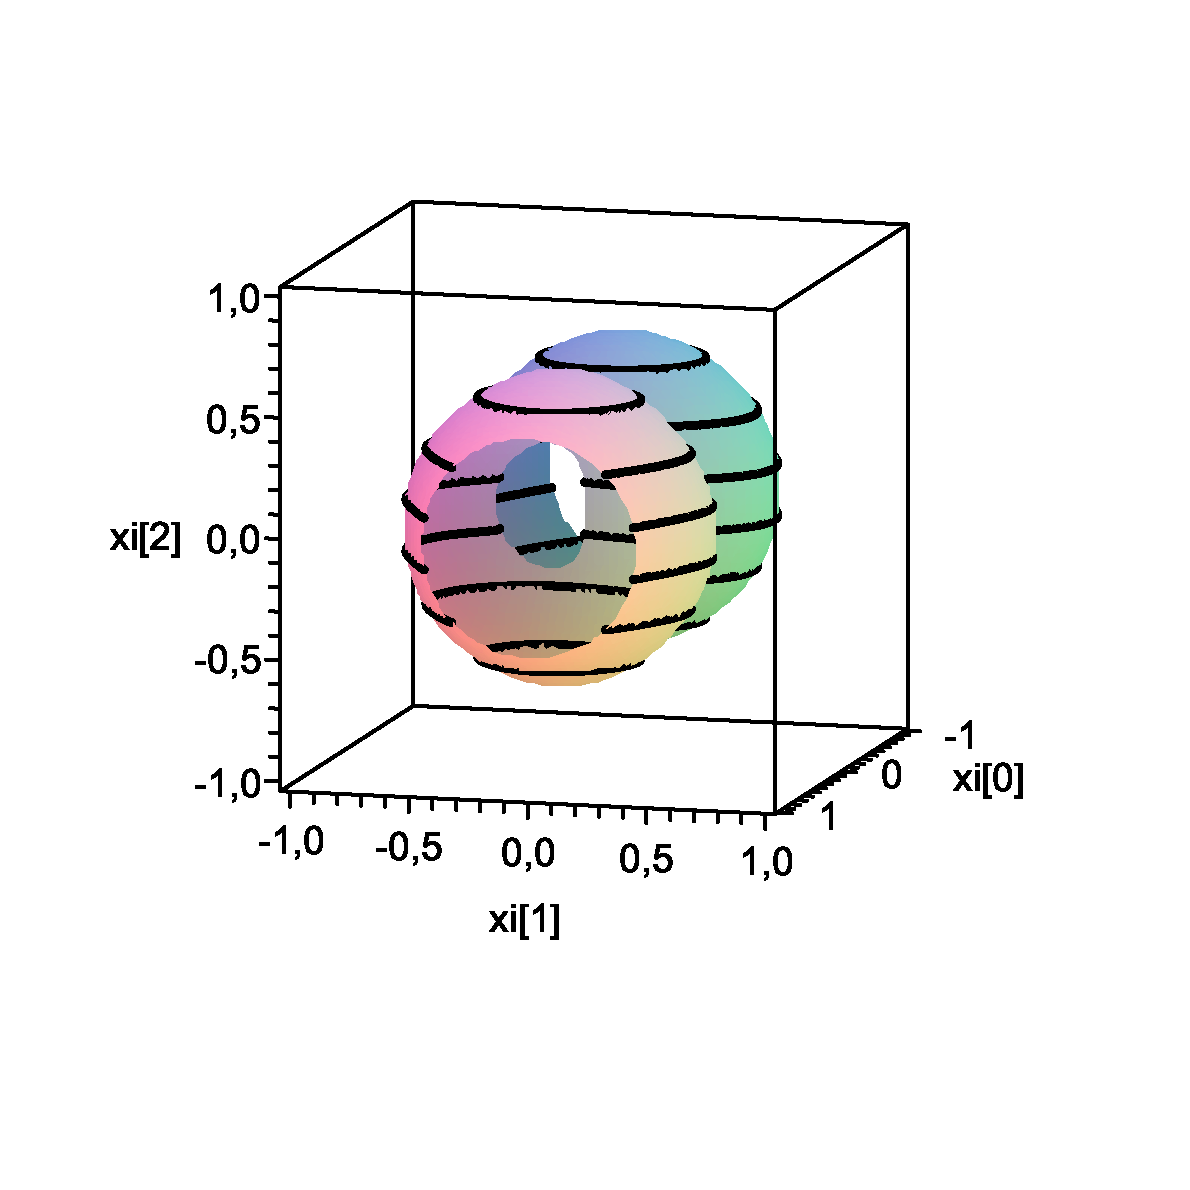
\includegraphics[width=0.3\textwidth,angle=0]{pic-res-2} \ \
	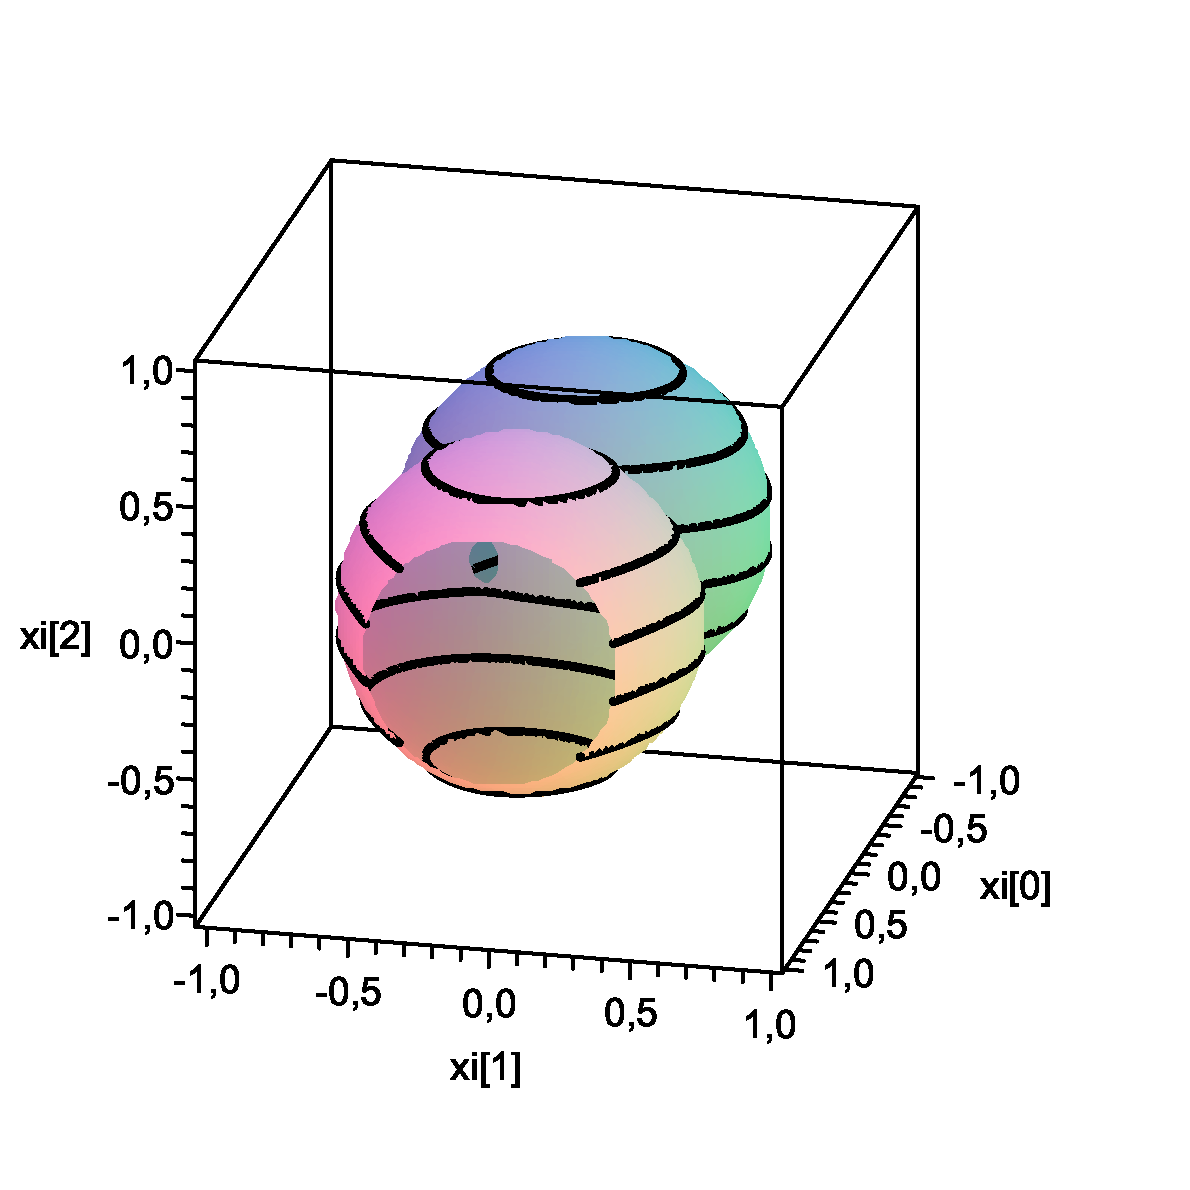
\includegraphics[width=0.3\textwidth,angle=0]{pic-res-4}  \ \
	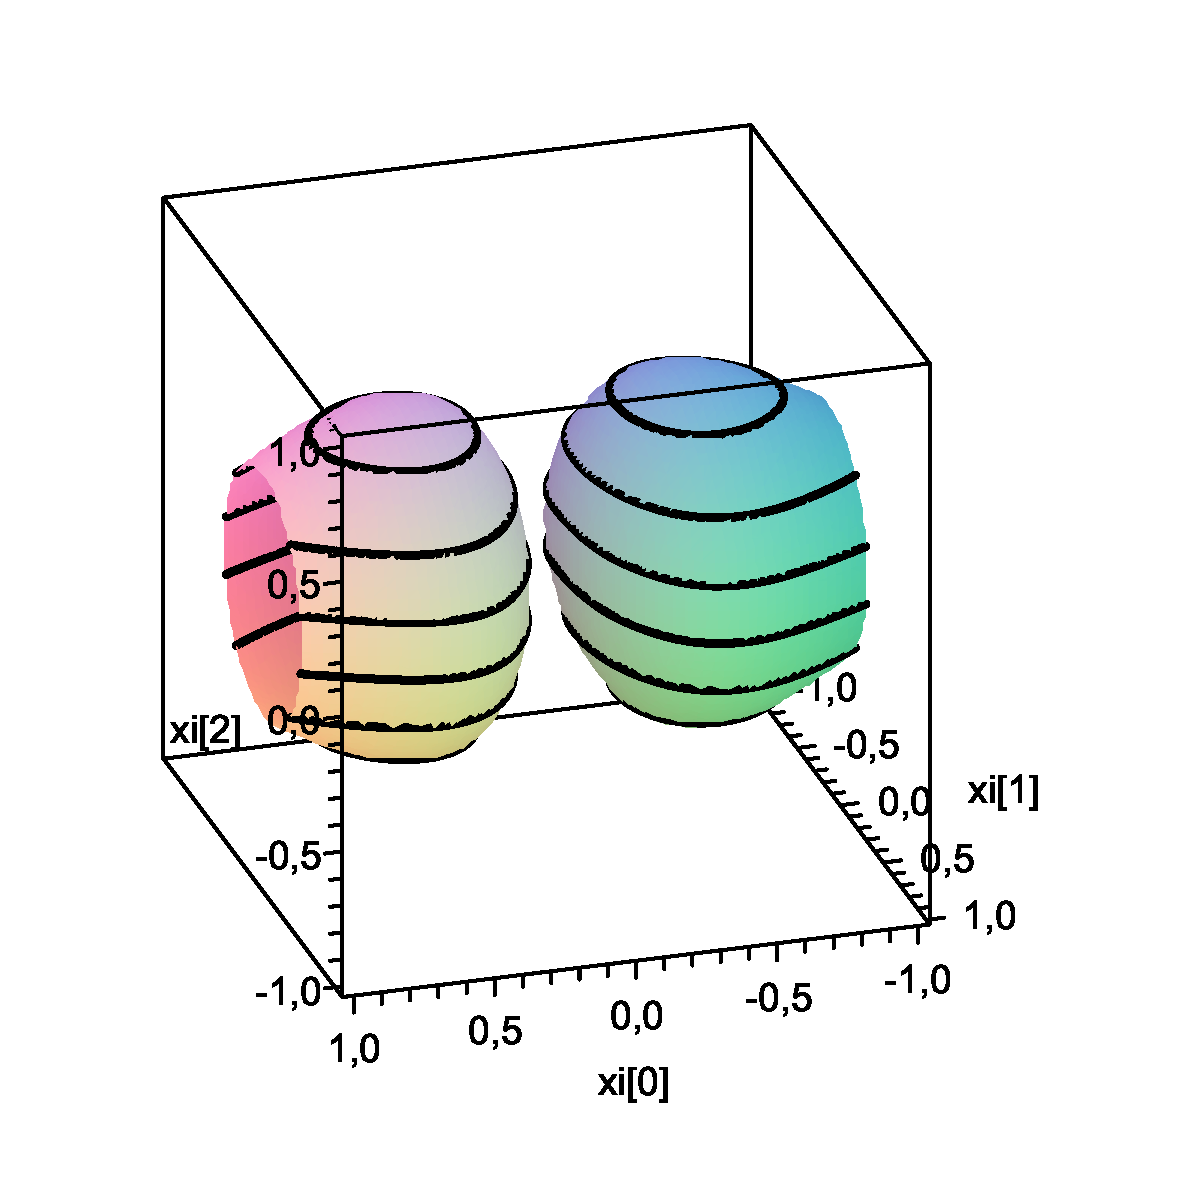
\includegraphics[width=0.3\textwidth,angle=0]{pic-res-5}
	\caption{
		Поверхности уровней второго приближения к
		ключевой функции маятника (при $\lambda = 1.01$,  $\ q_0=0\,, \ q_1=
		0.001\,,\ q_2= 0$\,, $W2=-0.003\,, \ 0.0038\,, \ 0.009$ ).
	}
\end{figure}



%%%%  ОФОРМЛЕНИЕ СПИСКА ЛИТЕРАТУРЫ %%%
\smallskip \centerline{\bf References}\nopagebreak

1. Арнольд В.И. Математические методы классической  механики /В.И.
Арнольд.  М.: Наука, 1989. - 472 с.


2. Красноселький М.А. Итерационный процесс с минимальными невязками
/ М.А. Красноселький , С.Г. Крейн //  Матем. сборник. 1952. Т.31
(73), в.2. - С.315-334.

3. Сапронов Ю.\;И.  Моделирование диффузорных течений
\linebreak
жидкости
посредством редуцированных уравнений  / Ю.И. Сапронов
// Вестник ЮУрГУ. Сер: Математическое моделирование и
программирование. 2014, том 7, № 2. - С.74-86.

4. Костина Т.И. Нелокальный анализ гладких вариационных задач с
параметрами / Т.И. Костина  // Канд. диссертация. Воронеж, ВГУ.
2011. - 122 с.
